\chapter{Particle Effects}
Particle Effects are the secret sauce to the graphics of your 2d game. They can
make graphics a lot more enjoyable. You now will learn how to create particle
effects in code and using Spritebuilder. However, before we discuss how to
create particle effects we need to understand which art is required for particle
effects.

\section{Art for particle effects}
Basically a particle effect (in \cocos{}) consists of a huge amount of Sprites
which are colored/blurred, or otherwise graphically manipulated, and moving in
patterns. This means the basic element of every particle effect is a texture for
a single particle. You can download the texture for our firt particle effect
here:TODO downloadlink. Two important things to note: the texture has a
transparent background and its structure is colored in grayscale colors. This
way the particle can be blended into any color. 
 \begin{figure}[H]
		\centering
		
\includegraphics[width=80pt]{images/particle_stars.png}     
		\caption{A classic texture for a particle effect.}
\end{figure}

\section{Particle Effect Basics}
\cocos{} provides a convinience class that allows to create particle effects
with a wide variety of parameters: CCParticleSystem.
In the appendix you can find a table that provides a brief description of each
parameter. However, it is a lot easiert to start with some examples.
\section{Particle Effects in \cocos{}}
In case you are not using Spritebuilder for your game - or you just want to
learn the underlying basics of creating custom particle effects, this chapter is
for you. We will learn how to build particle effects in code and using the
popular tool \textit{Particle Designer}.
\begin{lamp}[frametitle={Following this tutorial}]
If you want to implement this tutorial you need to start with this template
project: .We will add multiple scenes for different applications of particle
effects.
\end{lamp}
\label{subsec:particle effects in code}
\subsection{Configuring particle effects in code}
Most of the time you will want to design particle effects in a graphical editor
that provides a nice visual preview. However, to understand the basics we will
create our first particle effect in code (this is a great example from 
the cocos2d tests).

The steps we need to perform:
 \begin{itemize}
   \item create a CCParticleSystem
   \item select a particle texture
   \item set a duration for the particle effect
   \item set a huge amount of further, optional parameters
 \end{itemize}
\textbf{Now let's create our first particle effect.}
Add a new scene called \textit{ParticleEffectScene} to your project. You also
need to add a button to the \textit{MenuScene} that will allow us to present the
new \textit{ParticleEffectScene}.  
I won't provide the complete setup code (it's mostly
boring but can be found here: https://gist.github.com/Ben-G/8340545), here's the relevant part:
\begin{lstlisting}
    CCParticleSystem *emitter = [[CCParticleSystem alloc] initWithTotalParticles:50];
    emitter.texture = [[CCTextureCache sharedTextureCache] addImage: @"stars-grayscale.png"];
	emitter.duration = CCParticleSystemDurationInfinity;
    // lots of further parameters
\end{lstlisting}
Once the particle system is created, you add it as a child to your scene:
\begin{lstlisting}
    emitter.positionType = CCPositionTypeNormalized;
    codeParticleEffect.position = ccp(0.5f, 0.5f);
    [self addChild:emitter];
\end{lstlisting}
There is no need to start the particle effect - it is started as soon as it is
added to a parent node. However you can manually start/stop a particle system by
using the \textit{stopSystem} and \textit{resetSystem} methods. Now you can run
the app and you should see a particle effect in the middle of the scene. (TODO:
add screenshot) 
\subsection{Particle Effects with plists}
If you took some time to read through the setup in code
(https://gist.github.com/Ben-G/8340545) you have seen that it is very cumbersome
and nothing that actually should be part of your code base. Luckily \cocos{}
allows us to read particle effects from plist-files. You can fill these plists
manually, using the same parameters as when setting up particle systems in code
- however, the value of using plists only fully unfolds when you use graphical
editors to create your particle effects. Spritebuilder comes with an integrated
particle effect designer. If you don't use Spritebuilder, \textit{Particle
Designer}(http://particledesigner.71squared.com/) is the preferred tool to
create particle effects.
\subsection{Particle Effects in Particle Designer}
\subsection{Including particle effects in your gameplay}
Now that we have the basics it's the right time to add some best practices.
Mostly you will want to add particle effects dynamically to your scenes, based
on certain events such as collisions or explosions. Let's create a new class
called \textit{ParticleGamePlayScene}, again, don't forget to add a entry to
\textit{MenuScene} that let's you push the new scene.
We're going to build following scene:
 \begin{itemize}
   \item two spaceships, one at the left and one at the right edge of the sceen
   \item when a ship get's touched it fires a bullet at the other ship
   \item when a bullet hits another ship we play an explosion particle
   effect
\end{itemize}
To create this setting, we will add a lot of code that is not directly related
to particle effects. Let's discuss that code briefly, all of this takes place
in \textit{ParticleGamePlayScene.m}:
\begin{lstlisting}[title=examples/ParticleGamePlayScene.m]

@implementation ParticleGamePlayScene {
    CCSprite *leftShip;
    CCSprite *rightShip;
    NSMutableArray *bullets;
}

- (id)init
{
    self = [super init];
    
    if (self) {
        leftShip = [CCSprite spriteWithImageNamed:@"ship.png"];
        leftShip.anchorPoint = ccp(0.f, 0.5f);
        leftShip.position = ccp(0, self.contentSize.height/2);
        [self addChild:leftShip];
        
        rightShip = [CCSprite spriteWithImageNamed:@"ship.png"];
        rightShip.anchorPoint = ccp(1.f, 0.5f);
        rightShip.position = ccp(self.contentSize.width-rightShip.contentSize.width, self.contentSize.height/2);
        rightShip.scaleX = -1.f;
        [self addChild:rightShip];
        
        // enable touches
        self.userInteractionEnabled = TRUE;
        
        // initialize bullets array
        bullets = [NSMutableArray array];
    }
    
    return self;
}
\end{lstlisting}
Nothing special going on here. We create two ships, enable user interaction and
initialize a array that we use to keep track of active bullets.
Next, we need to react to touch input:
\begin{lstlisting}[title=examples/ParticleGamePlayScene.m]
#pragma mark - Touch Handling

- (void)touchBegan:(UITouch *)touch withEvent:(UIEvent *)event
{
    CGPoint touchPoint = [touch locationInNode:self];
    
    if (CGRectContainsPoint(leftShip.boundingBox, touchPoint)) {
        // fire left ship
        [self fireLeftShip];
    } else if (CGRectContainsPoint(rightShip.boundingBox, touchPoint)) {
        // fire right ship
        [self fireRightShip];
    }
}
\end{lstlisting}
We detect if the left or right ship has been touched by checking if the bounding
box of either ship contains the touch position. Depending on which ship has been
touched, we call the according firing method. 
\begin{lamp}[frametitle={Code Structure}] 
Please note that we usually would create a subclass for the ship to handle
touches and/or bullet spawning, however for the sake of readibility we reduce the amount of involved classes and handle everything in the scene itself.
\end{lamp}
Here are the firing methods: (TODO: improve positioning when anchor points are
fixed) 
\begin{lstlisting}[title=examples/ParticleGamePlayScene.m]
#pragma mark - Firing methods
- (void)fireLeftShip
{
    CCSprite *bullet = [CCSprite spriteWithImageNamed:@"bullet.png"];
    bullet.anchorPoint = ccp(0.f, 0.5f);
    bullet.position = ccp(leftShip.boundingBox.origin.x+leftShip.boundingBox.size.width, leftShip.position.y);
    [self addChild:bullet];
    CCAction *bulletMove = [CCActionMoveTo actionWithDuration:3.f position:ccp(self.contentSize.width, rightShip.position.y)];
    [bullet runAction:bulletMove];
    [bullets addObject:bullet];
}

- (void)fireRightShip
{
    CCSprite *bullet = [CCSprite spriteWithImageNamed:@"bullet.png"];
    bullet.scaleX = -1.f;
    bullet.anchorPoint = ccp(0.f, 0.5f);
    bullet.position = ccp(rightShip.boundingBox.origin.x-bullet.contentSize.width, rightShip.position.y);
    [self addChild:bullet];
    CCAction *bulletMove = [CCActionMoveTo actionWithDuration:3.f position:leftShip.position];
    [bullet runAction:bulletMove];
    [bullets addObject:bullet];
}
\end{lstlisting}
The firing methods take care of spawning bullets. We use \textit{CCActionMoveTo}
to shoot in the direction of the other ship. 

Now that we went through all of the
boilerplate code we get to the actually interesting part of our small project:
detecting collisions and launching particle effects.
For collision detection we use the \textit{update} method, that is called every
frame. To create particle effects, we use the code from \ref{subsec:particle
effects in code} with some slight modifications:
\begin{lstlisting}
#pragma mark - Collision Detection

- (void)update:(CCTime)delta
{
    for (int i = 0; i < [bullets count]; i++) {
        CCSprite *bullet = bullets[i];
        
        if (CGRectIntersectsRect(bullet.boundingBox, leftShip.boundingBox) || CGRectIntersectsRect(bullet.boundingBox, rightShip.boundingBox)) {
            [bullet removeFromParent];
            [bullets removeObjectAtIndex:i];
            CCParticleSystem *particleEffect = [self createParticleEffectInCode];
            particleEffect.position = bullet.position;
            [self addChild:particleEffect];
        }
    }
}
 
#pragma mark - Provide particle effect

- (CCParticleSystem *)createParticleEffectInCode
{
    CCParticleSystem *emitter = [[CCParticleSystem alloc] initWithTotalParticles:50];
	emitter.texture = [[CCTextureCache sharedTextureCache] addImage: @"stars-grayscale.png"];
	// duration
	emitter.duration = 1.f;
    emitter.autoRemoveOnFinish = TRUE;
	[...]
	return emitter;
}
\end{lstlisting}

\textbf{Collision
Detection.} We iterate through the bullets, determining if any bullet intersects one of the two ships. Once we detect a collision we remove the
bullet from the scene and the bullets array and create a particle effect at the
same position.

\textbf{Creating particle effect.} I stripped away all the visual setup. The two
important changes to the particle effect, compared to \ref{subsec:particle
effects in code} are setting the duration to 1 second and setting
\textit{autoRemoveOnFinish} to \textit{TRUE}. This means that once the particle
effect is added in the collision detection method it will run for 1 second and
after it completed it will automatically be removed from the scene. This means
we don't have to take care of cleaning the partical effect up manually.

If you run the project now, you should be able to fire bullets and you should
see particle effects every time a bullet collides with a ship.

\begin{figure}[H]
		\centering
		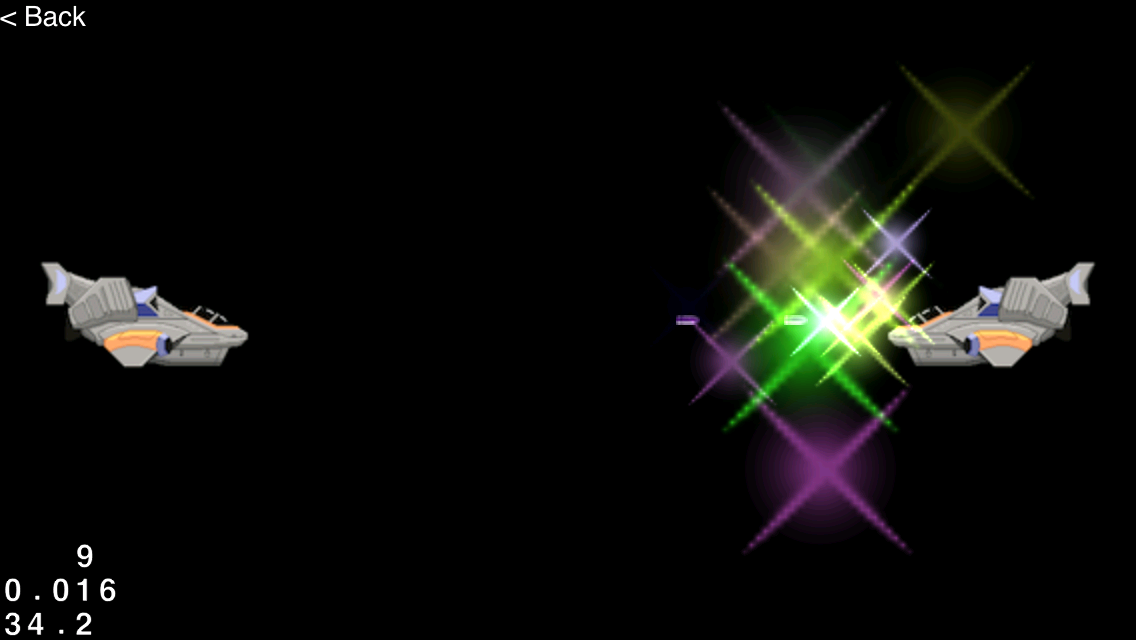
\includegraphics[width=275pt]{images/particles/particle_explosion.png}   
\end{figure}

Congratulations! Now you know how to dynamically add particle effects to your
game in \cocos{}. In the next chapter you will learn how to accomplish this in
Spritebuilder.

\section{Particle Effects in Spritebuilder}
Now that we understand the nature of particle effects and have implemented some
basics, we will take a look at how Spritebuilder works with particle effects.
Similar to the preceeding chapter we will start by statically adding particle
effects to a scene first and then will integrate particle effects
to our gameplay.
\textbf{First, let's get started by creating a new Spritebuilder project}.
First open the menu to add a new interface file: 
\begin{figure}[H]
		\centering
		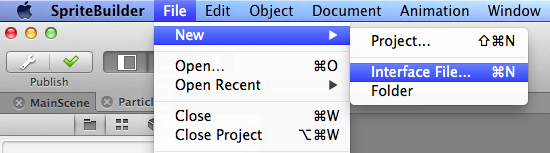
\includegraphics[width=275pt]{images/particles/Spritebuilder_ParticleEffect_Menu1.png}   
\end{figure}
Next, select \textit{Particles} as document type:
\begin{figure}[H]
		\centering
		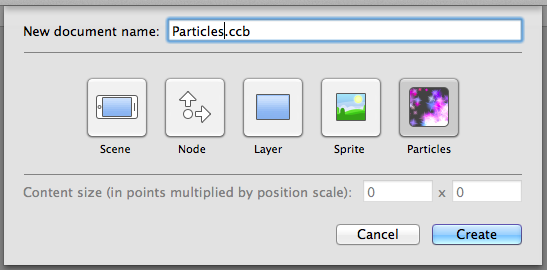
\includegraphics[width=275pt]{images/particles/Spritebuilder_ParticleEffect_Menu2.png}   
\end{figure}
Now you should see the newly created particle effect on your stage. To select
the node you can use the timeline and select the \textit{CCParticleSystemQuad}
(highlighted blue in the screenshot):
\begin{figure}[H]
		\centering
		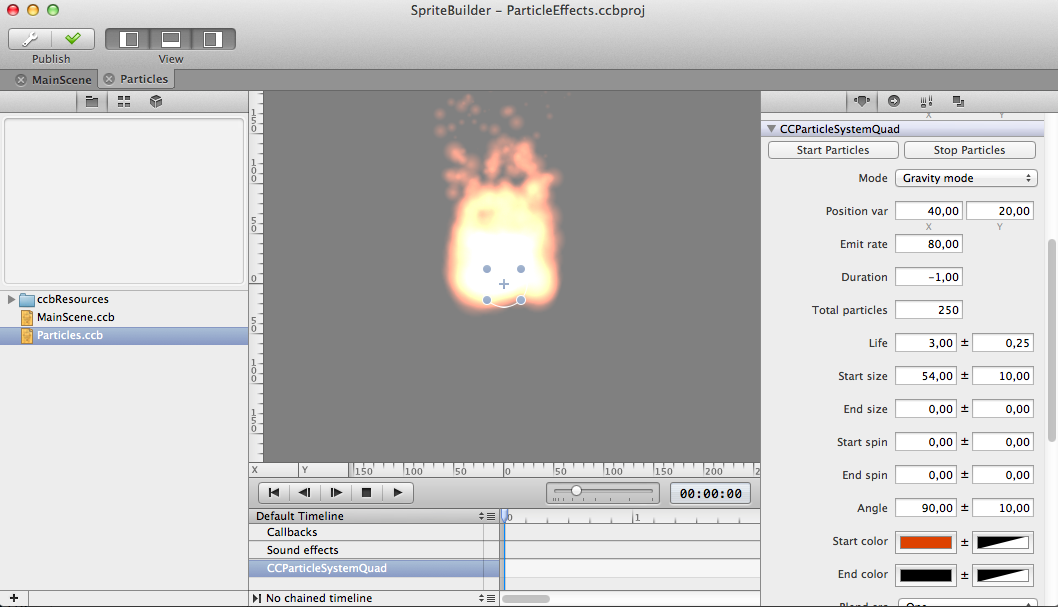
\includegraphics[width=375pt]{images/particles/Spritebuilder_ParticleEffect_CCB.png}   
		\caption{Stage with a default particle effect}
\end{figure}
In the inspector on the right you can see all (check if this is true) properties
that we have set in code previously. You can update them and get a live preview
of how they influence your particle effect. 

Spritebuilder comes with a nice library of template particle effects. You can
view them in the rightmost tab of the inspector:
\begin{figure}[H]
		\centering
		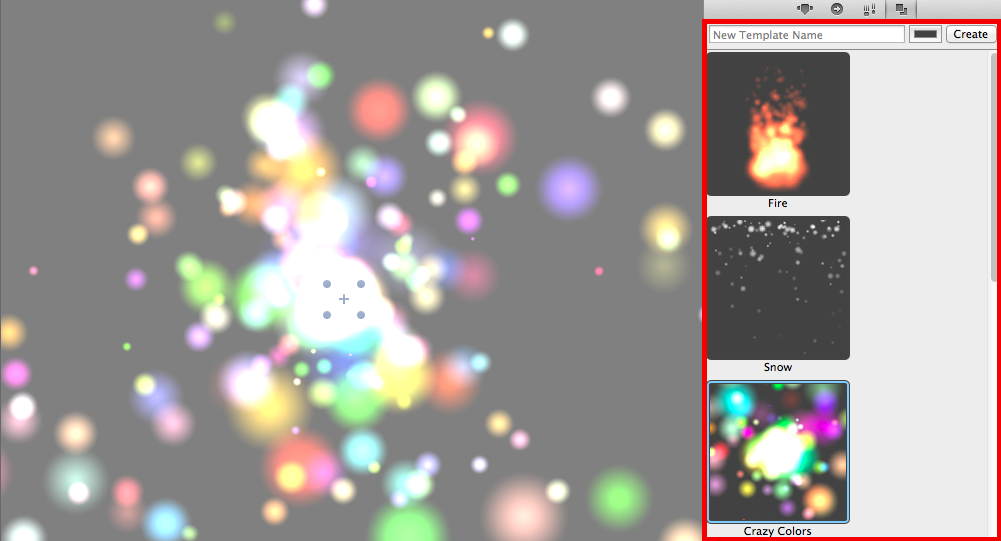
\includegraphics[width=375pt]{images/particles/Spritebuilder_ParticleEffect_Templates.png}   
		\caption{Spritebuilder provides many particle effect templates}
\end{figure}
to select one of the templates, simply double-click it.
\subsection{Adding the particle effect to your scene}
Spritebuilder creates a new CCB File for each of your particle effects. If you
want to add a particle effect to one of your gameplay scenes you need to add the
CCB File of the particle effect as a child. 
You can do this by dropping a \textit{Interface File} child node on your target
scene:
\begin{figure}[H]
		\centering
		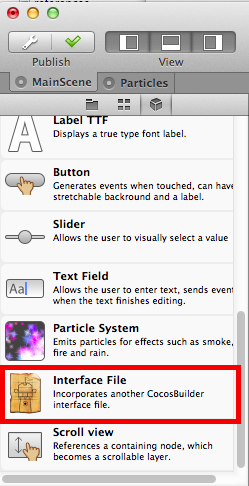
\includegraphics[width=70pt]{images/particles/Spritebuilder_ParticleEffect_AddInterfaceFile.png}   
		\caption{Interface Files let you include CCB Files in other CCB Files}
\end{figure}
Once the \textit{Interface File} node is added, you can choose which CCB File
shall be included. The inspector provides a dropdown with all available CCB
Files, here you can choose the CCB of your particle effect.
 \begin{figure}[H]
		\centering
		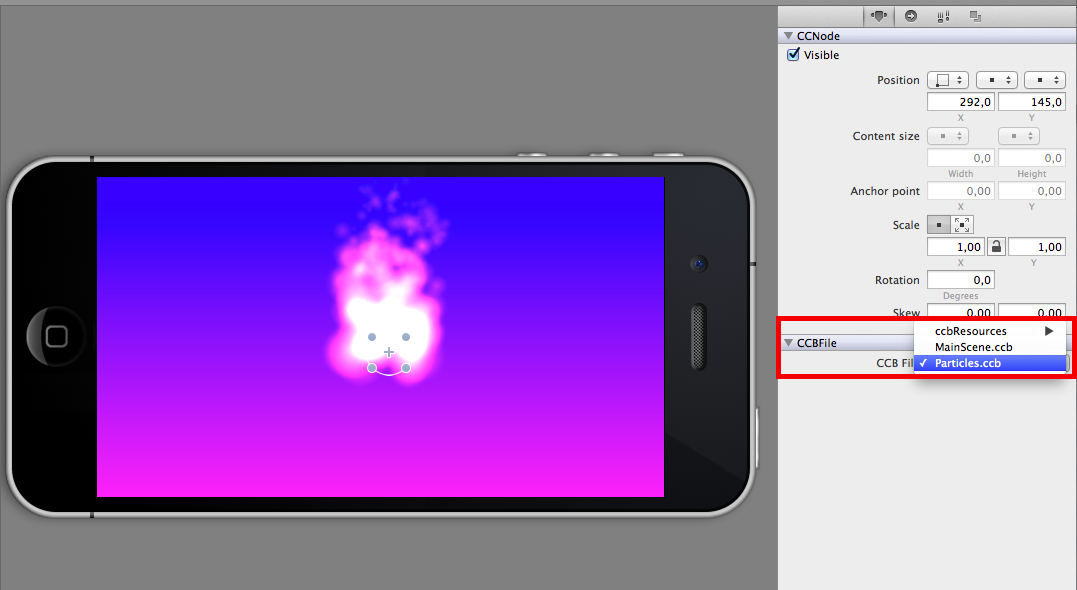
\includegraphics[width=375pt]{images/particles/Spritebuilder_ParticleEffect_InterfaceFile.png}
		\caption{In the dropdown of the inspector you can choose which CCB File
		should be included}
\end{figure}
Now you have succesfully added the particle effect to your scene. However,
mostly when you work with particle effects you will not add to your scene
statically, as we just did, but you will want them to appear when certain events
occur, e.g. collisions or explosions. In the next chapter we will take a look
how we can add particle effects to our gameplay - dynamically. 
\subsection{Including particle effects in your gameplay}
 
\section{Q and A: Let's solve some problems}
Once again, this section provides some practicle solutions to common problems:
\subsection{Q: I want to add multiple particle effects of the same type to my
scene} 